\section{Results}
\label{sec:results}

The thrust baseline result is obtained from the 1994 workflow with Iterative Bayesian
Unfolding at nominal $N_{\mathrm{iter}}=5$, including the hadronic event correction,
ISR correction, and all configured systematic reruns.
All 14 nominal and systematic unfolding jobs completed successfully.
The response matrix diagonal fraction is 0.332, indicating substantial migration between
reconstructed and generated thrust bins.

\subsection{Final unfolded thrust distribution}

\begin{figure}[t!]
\centering
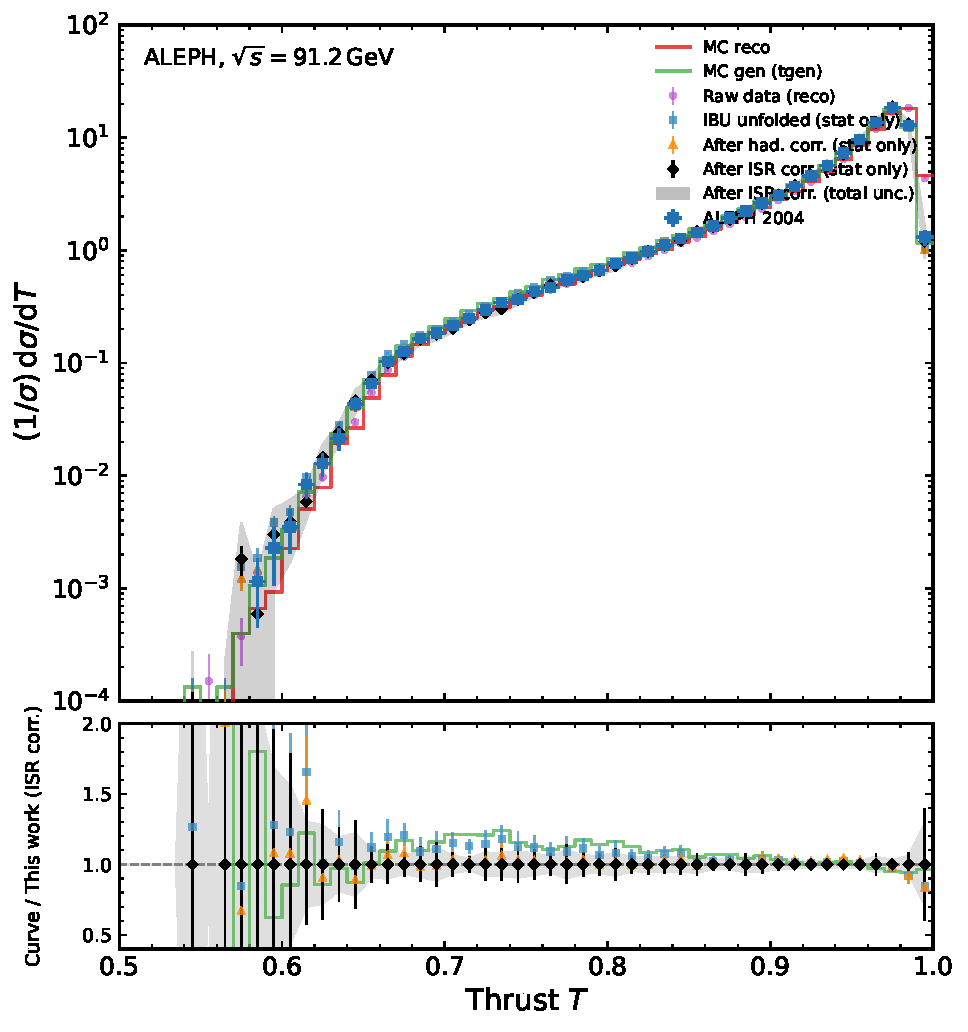
\includegraphics[width=0.49\textwidth]{figures/final_result_ratio_ours.pdf}%
\hfill%
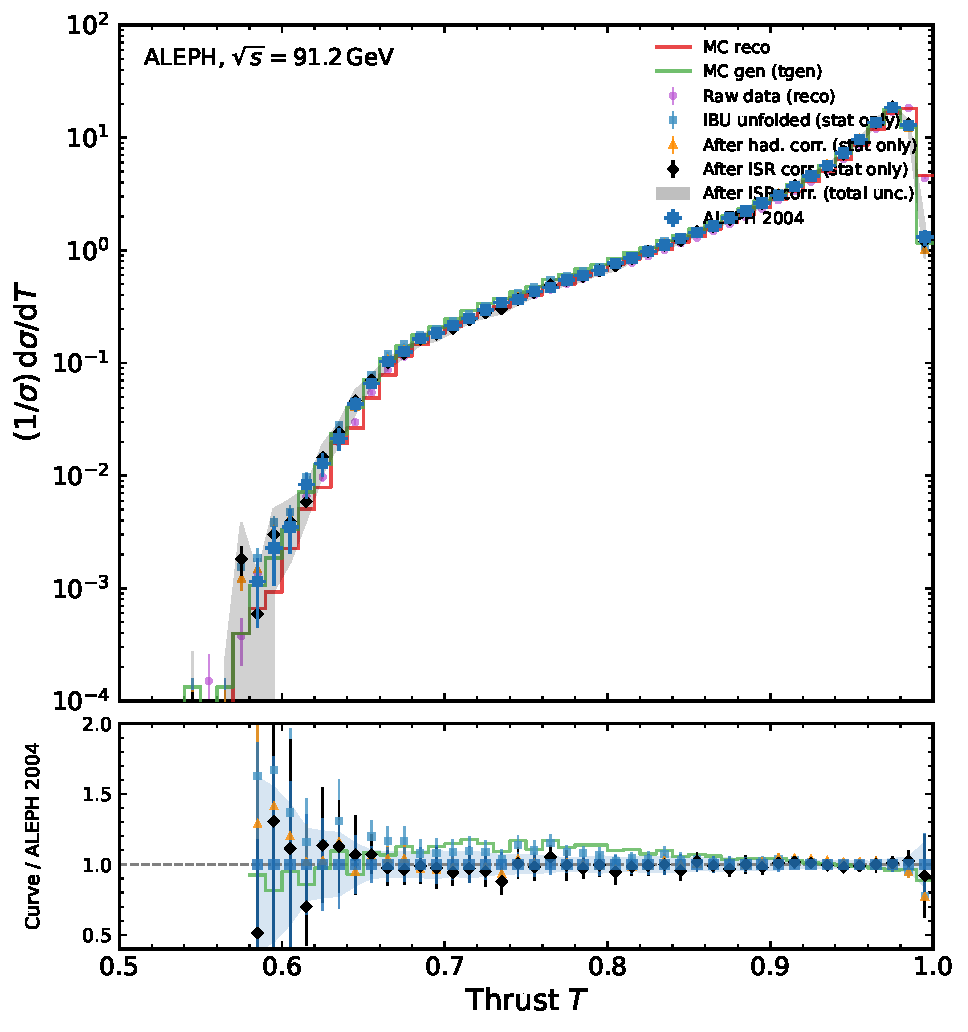
\includegraphics[width=0.49\textwidth]{figures/final_result_ratio_aleph.pdf}
\caption{Left: final unfolded thrust distribution showing all correction stages
(raw reco, MC reco, MC gen, IBU unfolded, after hadronic correction, after ISR correction)
compared to ALEPH 2004. The ratio panel is normalised to the fully corrected result of
this work; the gray band shows the total uncertainty envelope. Right: same stages with
the ratio panel normalised to the published ALEPH 2004 result. Agreement is good across
the bulk of the spectrum ($0.62\le T<0.99$); the elevated endpoint ratio ($1.30\pm0.27$)
is physically expected (soft-hadron sensitivity, hadronic/ISR correction growth,
normalisation convention differences).}
\label{fig:final_thrust_result}
\end{figure}

\begin{figure}[t!]
\centering
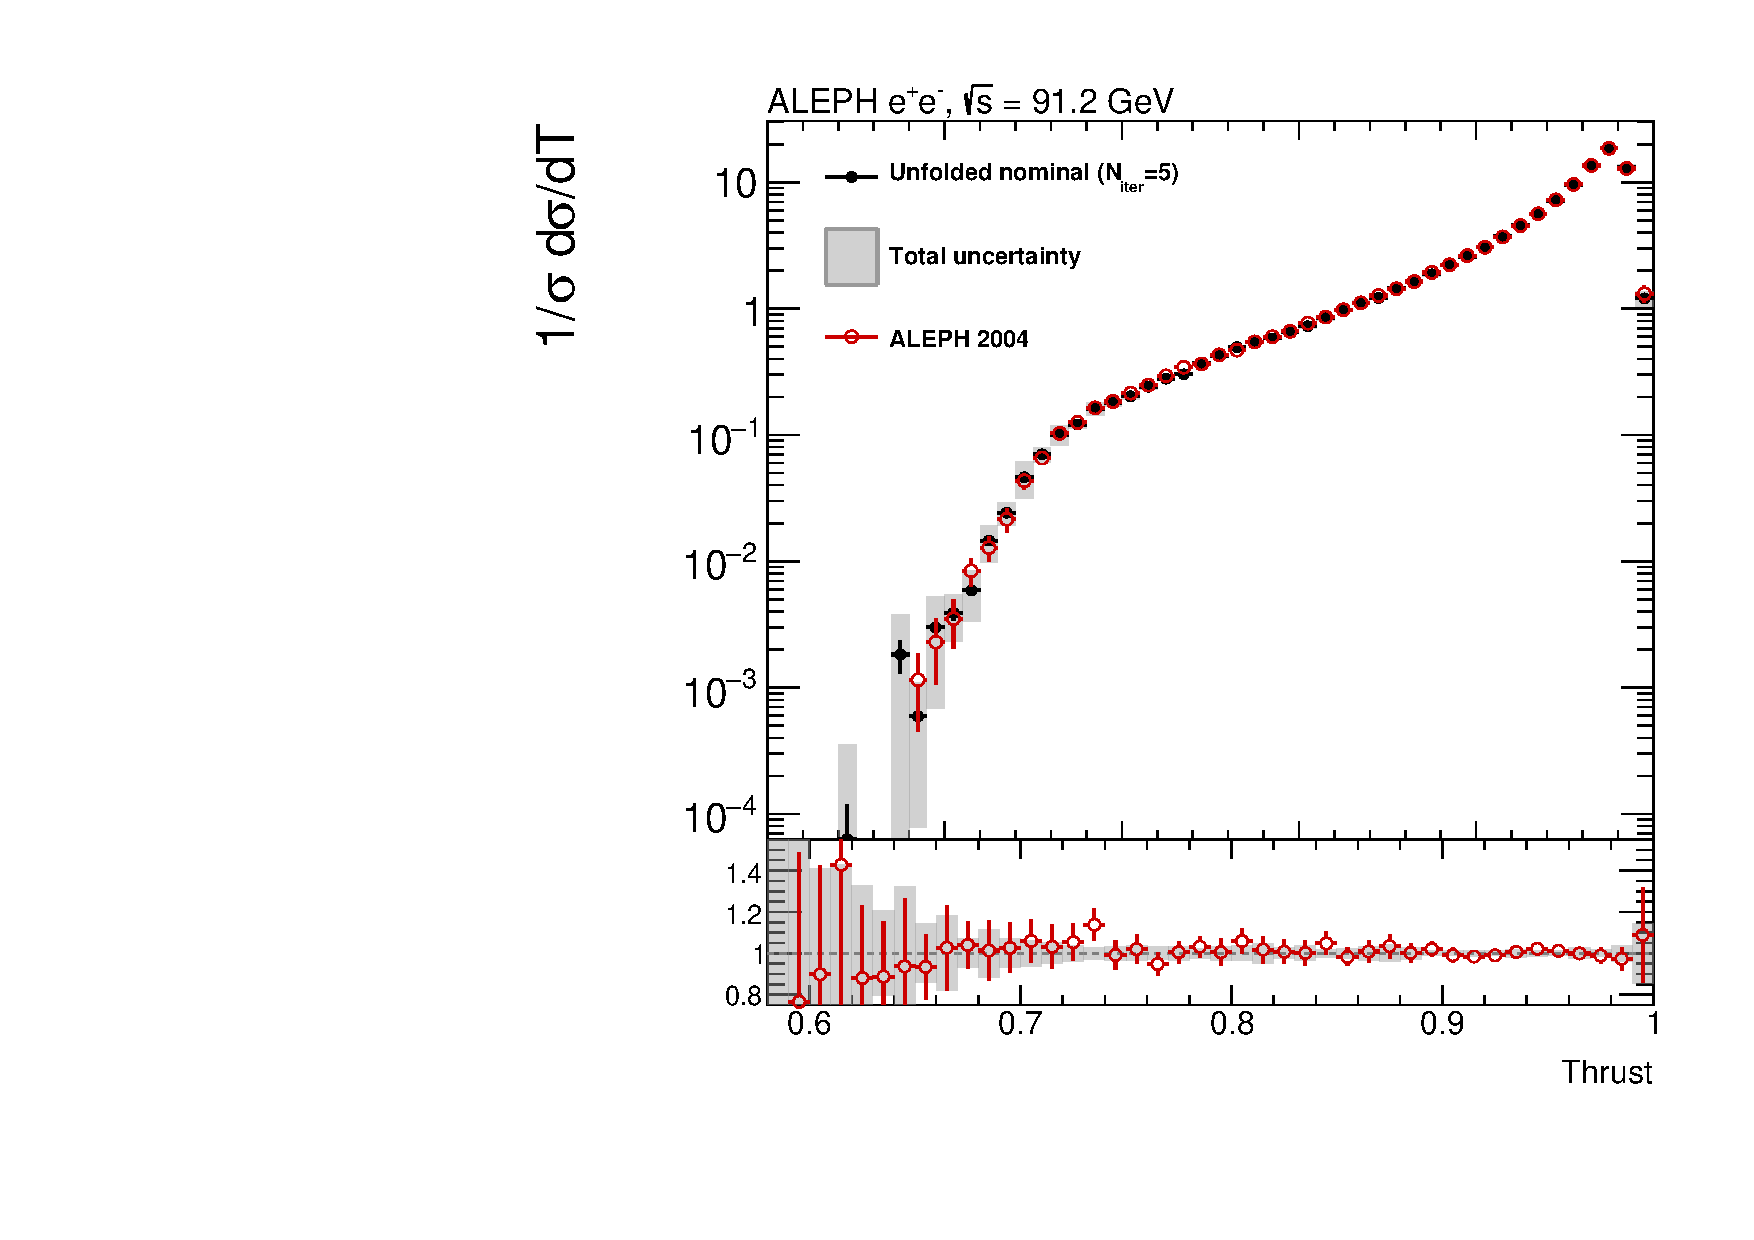
\includegraphics[width=0.48\textwidth]{figures/final_result_uncertainty_breakdown.pdf}%
\hfill%
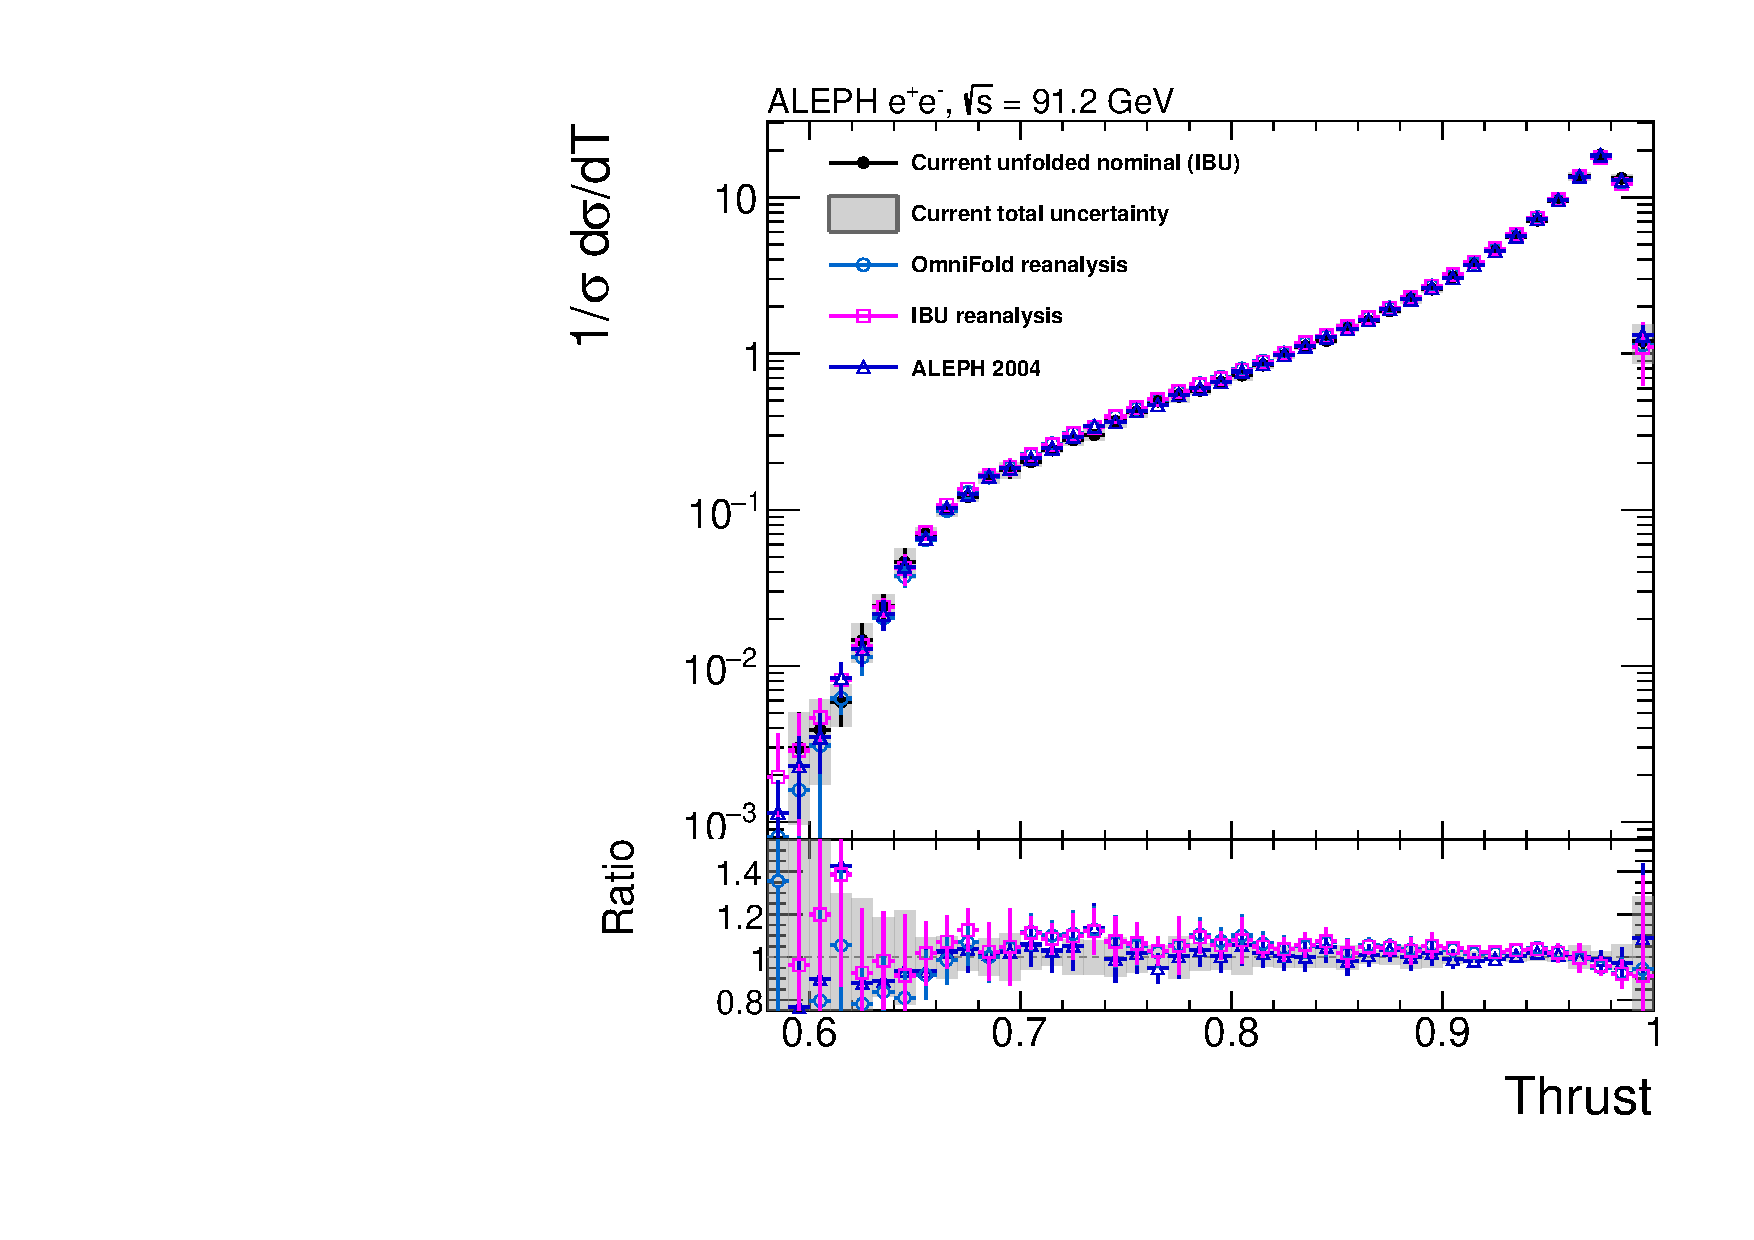
\includegraphics[width=0.48\textwidth]{figures/final_result_of_ibu_comparison.pdf}
\caption{Left: total uncertainty band for the final thrust result versus ALEPH 2004.
Right: comparison with OmniFold and prior IBU spectra; the ratio panel shows each
method relative to the current unfolded nominal. Compatibility metrics are
$\chi^2/\mathrm{ndf}=0.663$ (OmniFold), $0.421$ (prior IBU), and $0.361$ (ALEPH 2004),
evaluated over 42 bins using the diagonal of the total covariance.}
\label{fig:final_thrust_result_legacy}
\end{figure}

Figure~\ref{fig:final_thrust_result} (left) shows the unfolded spectrum with the total
uncertainty band and comparison to the published ALEPH 2004 result. Agreement is good
across the bulk of the spectrum ($0.62\le T<0.99$), with the largest discrepancy at
the endpoint ($0.99<T<1.00$, ratio $1.30\pm0.27$). This is physically expected: the
dijet limit is sensitive to MC modeling of soft hadrons, and the hadronic correction
$C_{\mathrm{had}}(j)$ and ISR correction $C_{\mathrm{ISR}}(j)$ carry growing
uncertainties there. Normalization convention differences between the current analysis
and the 2004 ALEPH publication also contribute at the endpoint.

Figure~\ref{fig:final_thrust_result} (right) shows direct comparison with OmniFold and
prior IBU spectra from the archived-data analysis program. Sub-unity $\chi^2/\mathrm{ndf}$
values reflect the conservative uncertainty model and positive off-diagonal correlations,
not overestimation. Differences are localized to the endpoint region.

\begin{figure}[t!]
\centering
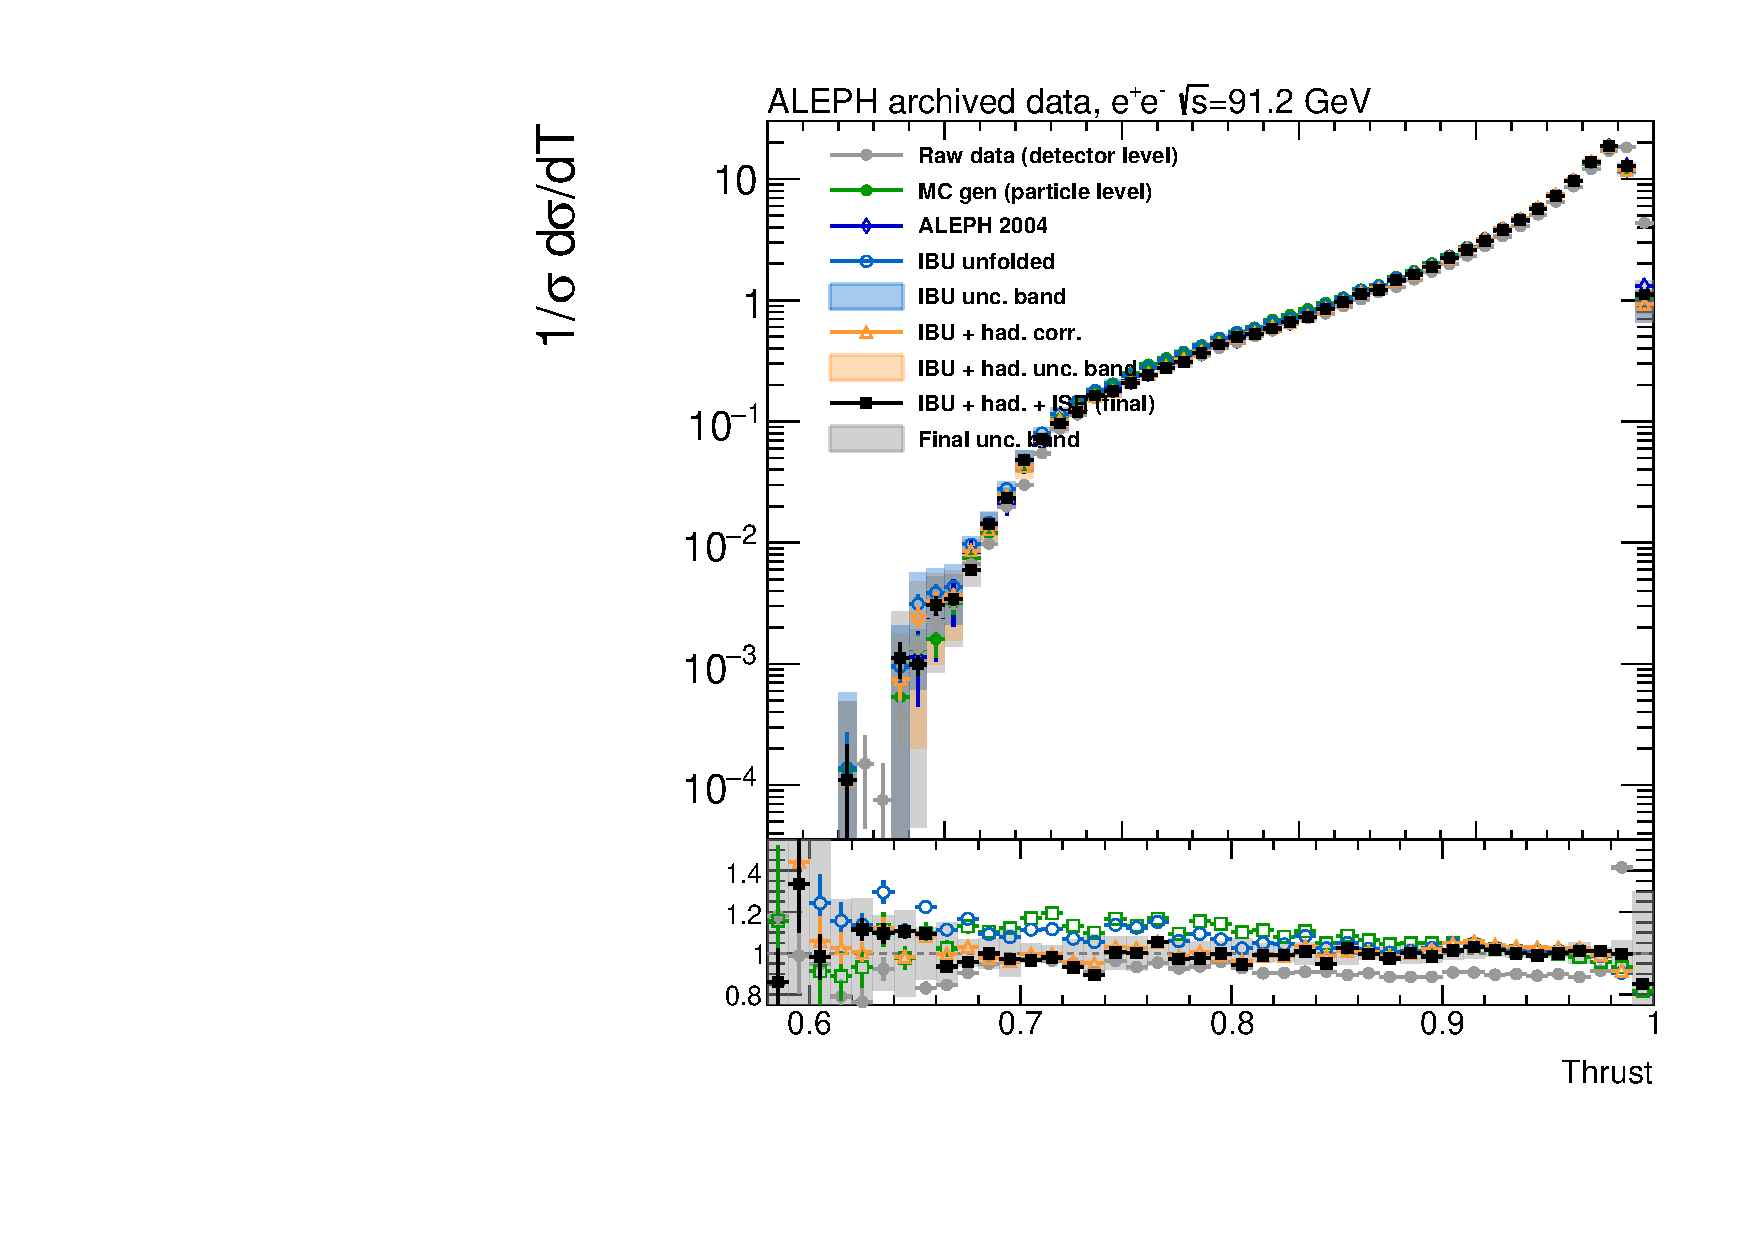
\includegraphics[width=0.49\textwidth]{figures/final_result_correction_stages.pdf}%
\hfill%
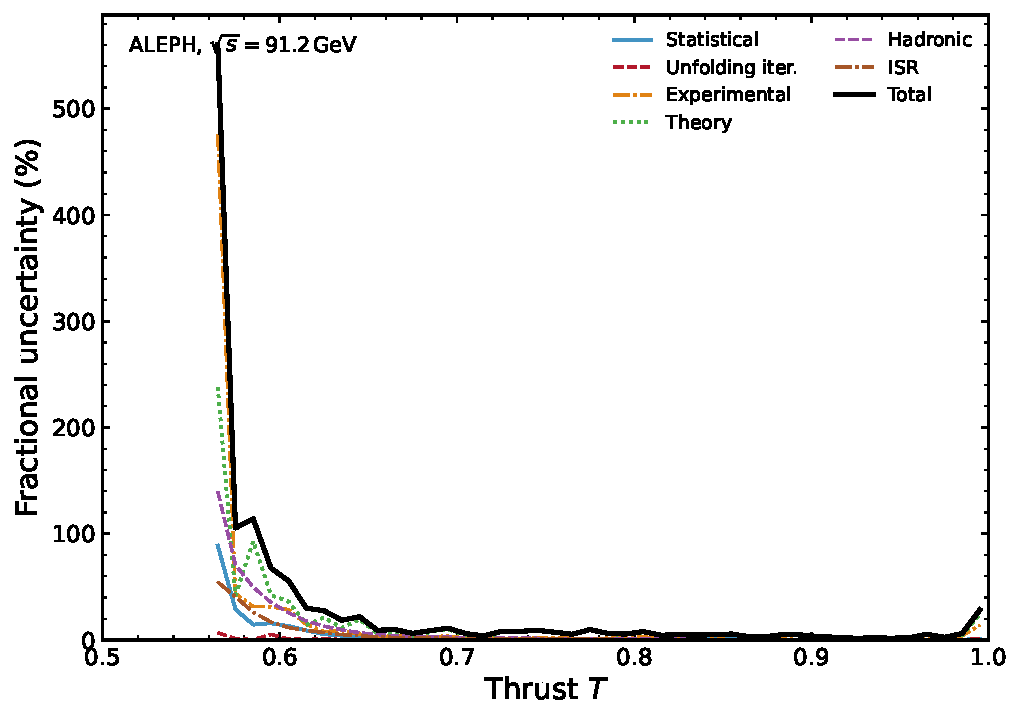
\includegraphics[width=0.49\textwidth]{figures/uncertainty_breakdown.pdf}
\caption{Left: all correction stages compared to ALEPH 2004, with ratio panel showing
each stage divided by the ALEPH 2004 result. The progression from IBU-only through
hadronic and ISR corrections is visible in the ratio panel. Right: fractional
per-component uncertainty as a function of thrust $T$. Theory dominates in the central
range; statistical and experimental components are sub-leading; ISR is small and nearly
flat.}
\label{fig:correction_stages_and_unc}
\end{figure}

The total correlation matrix for the combined result is shown in
Fig.~\ref{fig:final_total_correlation_matrix_sys}. The off-diagonal structure is
non-trivial and arises mainly from the unfolding of detector-level migration: it is
carried by the statistical (RooUnfold) covariance and by the systematic components that
inherit its correlation template. Under the nominal model the theory component enters as
a diagonal covariance (Sec.~\ref{sec:stat_covariance}) and therefore contributes only to
the per-bin variances, not to the bin-to-bin correlations. The off-diagonal correlations
remain non-negligible, so the full covariance matrix, rather than diagonal uncertainties
alone, must be used in any downstream fit or comparison.

\begin{figure}[t!]
\centering
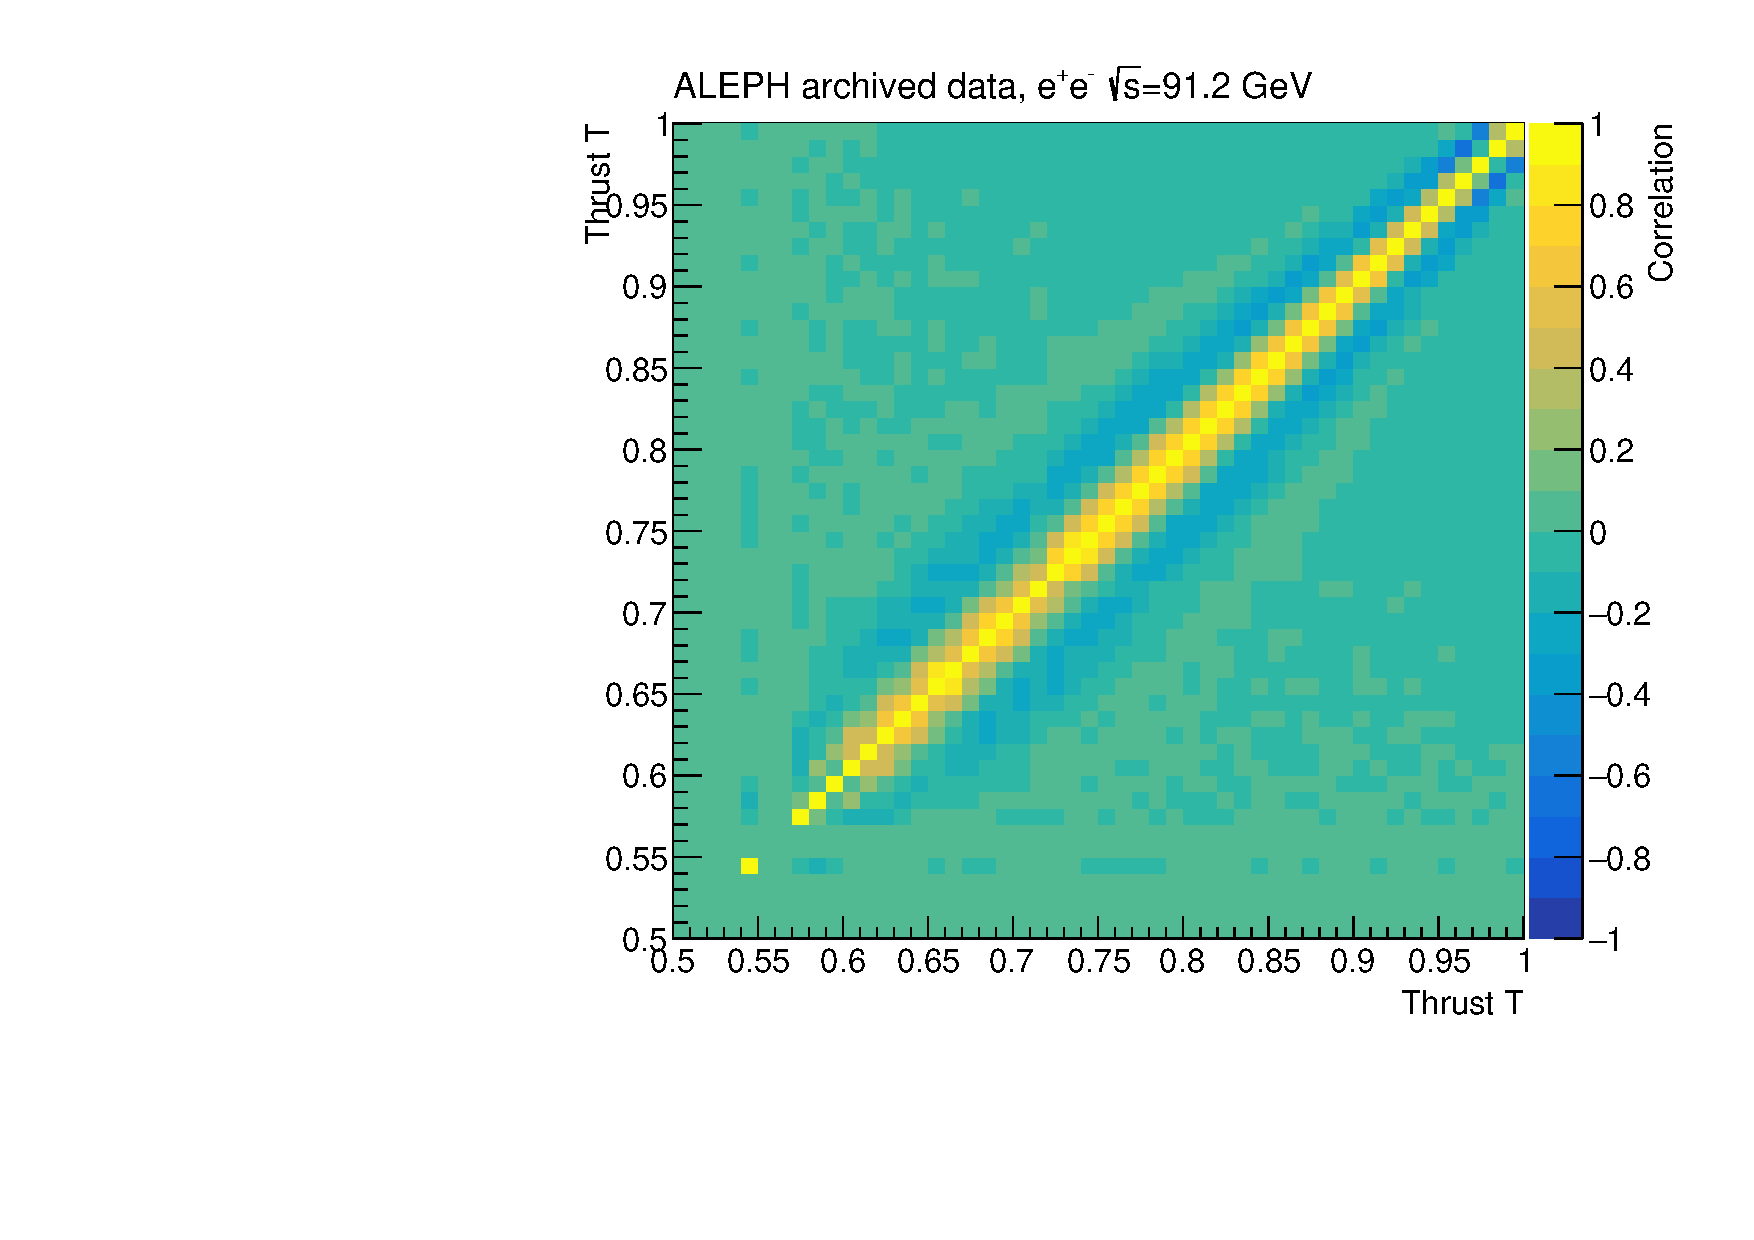
\includegraphics[width=\textwidth]{figures/matrix_total_correlation_final.pdf}
\caption{Total bin-to-bin correlation matrix for the final result, combining
statistical, unfolding-iteration, experimental, theory, hadronic-correction, and
ISR-correction components. The theory component enters as a diagonal covariance under
the nominal model, so it adds no off-diagonal correlation; the off-diagonal structure
is driven by the unfolding/response migration carried by the statistical covariance and
the components that inherit its correlation template.}
\label{fig:final_total_correlation_matrix_sys}
\end{figure}

The numerical per-bin uncertainty breakdown is given in
Tables~\ref{tab:per_bin_uncertainty}--\ref{tab:per_bin_uncertainty_breakdown_comparison},
listing all component contributions and the total for each thrust bin.

\begin{table}[t!]
\centering
\scriptsize
\begin{tabular}{c r c c c c c c}
\hline
$T$ range & $(1/\sigma)\,\mathrm{d}\sigma/\mathrm{d}T$ & Stat. & Iter. & Exp. & Theory & Had.\ corr. & Total \\
 & & [\%] & [\%] & [\%] & [\%] & [\%] & [\%] \\
\hline
{[0.56,0.57)} & $6.30\times10^{-5}$ & 88.8 & 6.9 & 467.8 & 67.7 & 139.7 & 500.9 \\
{[0.57,0.58)} & 0.0012 & 28.8 & 1.2 & 46.7 & 38.3 & 70.5 & 97.2 \\
{[0.58,0.59)} & 0.0015 & 14.5 & 0.4 & 25.0 & 59.5 & 49.6 & 82.7 \\
{[0.59,0.60)} & 0.0032 & 15.8 & 5.2 & 35.8 & 53.5 & 35.5 & 75.3 \\
{[0.60,0.61)} & 0.0042 & 13.1 & 0.9 & 25.9 & 7.1 & 25.5 & 39.3 \\
{[0.61,0.62)} & 0.0085 & 8.9 & 0.6 & 17.1 & 32.9 & 17.8 & 42.1 \\
{[0.62,0.63)} & 0.0131 & 5.5 & 0.9 & 7.3 & 27.7 & 13.0 & 32.0 \\
{[0.63,0.64)} & 0.0248 & 4.1 & 0.6 & 8.2 & 14.8 & 9.6 & 19.9 \\
{[0.64,0.65)} & 0.0411 & 3.1 & 0.5 & 6.3 & 30.5 & 6.9 & 32.0 \\
{[0.65,0.66)} & 0.0695 & 2.2 & 0.6 & 2.6 & 12.6 & 5.0 & 14.0 \\
{[0.66,0.67)} & 0.1068 & 1.9 & 0.8 & 3.8 & 16.9 & 3.9 & 17.9 \\
{[0.67,0.68)} & 0.1305 & 1.5 & 0.3 & 2.7 & 4.7 & 3.4 & 6.6 \\
{[0.68,0.69)} & 0.1587 & 1.5 & 0.1 & 2.6 & 10.6 & 2.9 & 11.4 \\
{[0.69,0.70)} & 0.1776 & 1.3 & 0.5 & 4.3 & 4.3 & 2.7 & 6.7 \\
{[0.70,0.71)} & 0.2087 & 1.2 & 0.5 & 1.4 & 5.2 & 2.4 & 6.0 \\
{[0.71,0.72)} & 0.2448 & 1.2 & 0.7 & 2.4 & 3.3 & 2.1 & 4.8 \\
{[0.72,0.73)} & 0.2876 & 1.0 & 0.3 & 1.1 & 2.6 & 1.9 & 3.6 \\
{[0.73,0.74)} & 0.3210 & 1.0 & 0.2 & 1.2 & 1.4 & 1.8 & 2.8 \\
{[0.74,0.75)} & 0.3792 & 0.9 & 0.2 & 1.9 & 1.8 & 1.6 & 3.2 \\
{[0.75,0.76)} & 0.4332 & 0.9 & 0.6 & 2.3 & 1.7 & 1.5 & 3.4 \\
{[0.76,0.77)} & 0.4958 & 0.8 & 0.5 & 1.5 & 1.9 & 1.4 & 3.0 \\
{[0.77,0.78)} & 0.5504 & 0.8 & 0.2 & 0.5 & 2.8 & 1.2 & 3.2 \\
{[0.78,0.79)} & 0.5994 & 0.7 & 0.1 & 1.8 & 0.9 & 1.1 & 2.4 \\
{[0.79,0.80)} & 0.6550 & 0.8 & 0.4 & 3.0 & 1.1 & 1.0 & 3.4 \\
{[0.80,0.81)} & 0.7399 & 0.7 & 0.5 & 3.0 & 1.6 & 0.9 & 3.6 \\
{[0.81,0.82)} & 0.8395 & 0.7 & 0.3 & 1.4 & 4.4 & 0.8 & 4.8 \\
{[0.82,0.83)} & 0.9697 & 0.6 & 0.2 & 0.9 & 2.3 & 0.8 & 2.7 \\
{[0.83,0.84)} & 1.14 & 0.6 & 0.3 & 2.0 & 3.0 & 0.7 & 3.7 \\
{[0.84,0.85)} & 1.26 & 0.6 & 0.3 & 1.4 & 1.1 & 0.6 & 1.9 \\
{[0.85,0.86)} & 1.45 & 0.5 & 0.0 & 0.3 & 2.2 & 0.5 & 2.3 \\
{[0.86,0.87)} & 1.64 & 0.5 & 0.1 & 1.3 & 3.0 & 0.4 & 3.3 \\
{[0.87,0.88)} & 1.89 & 0.5 & 0.2 & 1.6 & 3.7 & 0.4 & 4.1 \\
{[0.88,0.89)} & 2.23 & 0.5 & 0.2 & 1.0 & 2.6 & 0.3 & 2.9 \\
{[0.89,0.90)} & 2.67 & 0.4 & 0.1 & 0.4 & 1.0 & 0.2 & 1.2 \\
{[0.90,0.91)} & 3.20 & 0.4 & 0.1 & 1.2 & 0.4 & 0.1 & 1.3 \\
{[0.91,0.92)} & 3.86 & 0.4 & 0.2 & 1.1 & 0.8 & 0.1 & 1.4 \\
{[0.92,0.93)} & 4.70 & 0.4 & 0.1 & 0.9 & 0.5 & 0.0 & 1.1 \\
{[0.93,0.94)} & 5.79 & 0.3 & 0.1 & 1.6 & 0.9 & 0.1 & 1.9 \\
{[0.94,0.95)} & 7.40 & 0.3 & 0.2 & 1.1 & 0.7 & 0.1 & 1.4 \\
{[0.95,0.96)} & 9.79 & 0.3 & 0.1 & 0.8 & 0.6 & 0.2 & 1.1 \\
{[0.96,0.97)} & 13.86 & 0.2 & 0.1 & 2.3 & 1.0 & 0.3 & 2.5 \\
{[0.97,0.98)} & 18.46 & 0.2 & 0.3 & 1.5 & 0.5 & 0.4 & 1.6 \\
{[0.98,0.99)} & 12.18 & 0.3 & 0.2 & 3.9 & 0.7 & 0.3 & 4.0 \\
{[0.99,1.00)} & 1.01 & 1.0 & 1.6 & 14.1 & 3.1 & 0.7 & 14.5 \\
\hline
\end{tabular}
\normalsize
\caption{Per-bin fractional uncertainties across the full measurement range ($0.55 \leq T < 1.0$). The second column gives the nominal unfolded $(1/\sigma)\,\mathrm{d}\sigma/\mathrm{d}T$ value; all remaining columns are absolute fractional uncertainties in percent. Bins with zero nominal spectrum (dashes) are below threshold. \textit{Exp.} denotes the total experimental component (track/event and neutral sub-components combined in quadrature), and \textit{Had.\ corr.} denotes the hadronic event-selection correction uncertainty.}
\label{tab:per_bin_uncertainty}
\end{table}

\begin{table}[t!]
\centering
\scriptsize
\begin{tabular}{c r r r r}
\hline
$T$ range & Our $(1/\sigma)\,\mathrm{d}\sigma/\mathrm{d}T$ & Our total unc.\ [\%] & ALEPH 2004 $(1/\sigma)\,\mathrm{d}\sigma/\mathrm{d}T$ & ALEPH 2004 total unc.\ [\%] \\
\hline
% {[0.54,0.55)} & 0.0001096 & 365.0 & \multicolumn{1}{c}{---} & \multicolumn{1}{c}{---} \\
% {[0.57,0.58)} & 0.001128 & 157.9 & \multicolumn{1}{c}{---} & \multicolumn{1}{c}{---} \\
{[0.58,0.59)} & 0.0009897 & 103.8 & 0.00115 & 61.2 \\
{[0.59,0.60)} & 0.003057 & 80.1 & 0.00229 & 54.1 \\
{[0.60,0.61)} & 0.003443 & 66.9 & 0.0035 & 41.7 \\
{[0.61,0.62)} & 0.005924 & 31.5 & 0.00839 & 25.0 \\
{[0.62,0.63)} & 0.0143 & 29.6 & 0.01283 & 23.1 \\
{[0.63,0.64)} & 0.02354 & 20.0 & 0.02148 & 21.9 \\
{[0.64,0.65)} & 0.04787 & 21.4 & 0.0433 & 14.4 \\
{[0.65,0.66)} & 0.07177 & 13.3 & 0.06556 & 9.2 \\
{[0.66,0.67)} & 0.09626 & 15.4 & 0.1028 & 8.5 \\
{[0.67,0.68)} & 0.1203 & 7.4 & 0.1258 & 8.7 \\
{[0.68,0.69)} & 0.1637 & 7.9 & 0.164 & 8.7 \\
{[0.69,0.70)} & 0.1792 & 11.6 & 0.1842 & 9.5 \\
{[0.70,0.71)} & 0.2068 & 5.2 & 0.2142 & 7.6 \\
{[0.71,0.72)} & 0.2431 & 4.4 & 0.2481 & 9.1 \\
{[0.72,0.73)} & 0.2743 & 6.8 & 0.2943 & 7.5 \\
{[0.73,0.74)} & 0.3073 & 9.3 & 0.3435 & 6.2 \\
{[0.74,0.75)} & 0.3668 & 8.2 & 0.3654 & 6.0 \\
{[0.75,0.76)} & 0.4313 & 8.5 & 0.4309 & 6.0 \\
{[0.76,0.77)} & 0.4948 & 6.1 & 0.4692 & 4.9 \\
{[0.77,0.78)} & 0.5304 & 7.1 & 0.5458 & 4.2 \\
{[0.78,0.79)} & 0.5847 & 6.1 & 0.5994 & 4.2 \\
{[0.79,0.80)} & 0.6593 & 5.8 & 0.6609 & 5.6 \\
{[0.80,0.81)} & 0.7255 & 7.3 & 0.768 & 4.6 \\
{[0.81,0.82)} & 0.8486 & 4.7 & 0.857 & 4.3 \\
{[0.82,0.83)} & 0.9727 & 4.2 & 0.9808 & 5.1 \\
{[0.83,0.84)} & 1.122 & 5.5 & 1.113 & 5.0 \\
{[0.84,0.85)} & 1.206 & 4.8 & 1.27 & 4.9 \\
{[0.85,0.86)} & 1.476 & 5.4 & 1.439 & 3.8 \\
{[0.86,0.87)} & 1.632 & 3.3 & 1.639 & 4.0 \\
{[0.87,0.88)} & 1.885 & 3.4 & 1.935 & 3.9 \\
{[0.88,0.89)} & 2.232 & 4.8 & 2.23 & 3.4 \\
{[0.89,0.90)} & 2.589 & 4.5 & 2.631 & 3.2 \\
{[0.90,0.91)} & 3.102 & 3.0 & 3.062 & 3.3 \\
{[0.91,0.92)} & 3.815 & 2.8 & 3.702 & 2.2 \\
{[0.92,0.93)} & 4.623 & 1.8 & 4.547 & 2.3 \\
{[0.93,0.94)} & 5.64 & 2.1 & 5.645 & 2.2 \\
{[0.94,0.95)} & 7.199 & 1.6 & 7.277 & 1.7 \\
{[0.95,0.96)} & 9.628 & 2.1 & 9.63 & 1.7 \\
{[0.96,0.97)} & 13.74 & 5.2 & 13.6 & 1.7 \\
{[0.97,0.98)} & 18.77 & 2.6 & 18.57 & 3.7 \\
{[0.98,0.99)} & 12.84 & 6.0 & 12.89 & 4.1 \\
{[0.99,1.00)} & 1.115 & 29.8 & 1.312 & 15.4 \\
\hline
\end{tabular}
\normalsize
\caption{Comparison of the nominal unfolded $(1/\sigma)\,\mathrm{d}\sigma/\mathrm{d}T$ and total fractional uncertainty with the published ALEPH 2004 result (HEPData ins:636645, Table~54) for bins with non-zero unfolded spectrum. The ALEPH 2004 total uncertainty combines statistical, sys$_1$, and sys$_2$ components in quadrature.}
\label{tab:per_bin_uncertainty_aleph}
\end{table}

\begin{table}[t!]
\centering
\scriptsize
\resizebox{\textwidth}{!}{%
\begin{tabular}{c  r r r r  r r r r  r r}
\hline
& \multicolumn{2}{c}{$(1/\sigma)\,\mathrm{d}\sigma/\mathrm{d}T$}
 & \multicolumn{2}{c}{Stat.\ [\%]}
 & \multicolumn{2}{c}{Exp.\ / Sys.\,1 [\%]}
 & \multicolumn{2}{c}{Theory\,/ Sys.\,2 [\%]}
 & \multicolumn{2}{c}{Total [\%]} \\
\cline{2-3}\cline{4-5}\cline{6-7}\cline{8-9}\cline{10-11}
$T$ range & Ours & ALEPH & Ours & ALEPH & Ours & ALEPH & Ours & ALEPH & Ours & ALEPH \\
\hline
% {[0.54,0.55)} & 0.0001096 & \multicolumn{1}{c}{---} & 96.3 & \multicolumn{1}{c}{---} & 289.4 & \multicolumn{1}{c}{---} & 93.6 & \multicolumn{1}{c}{---} & 348.3 & \multicolumn{1}{c}{---} \\
% {[0.57,0.58)} & 0.001128 & \multicolumn{1}{c}{---} & 33.0 & \multicolumn{1}{c}{---} & 23.2 & \multicolumn{1}{c}{---} & 112.7 & \multicolumn{1}{c}{---} & 141.3 & \multicolumn{1}{c}{---} \\
{[0.58,0.59)} & 0.0009897 & 0.00115 & 18.9 & 29.6 & 42.6 & 45.2 & 65.4 & 28.7 & 95.5 & 61.2 \\
{[0.59,0.60)} & 0.003057 & 0.00229 & 17.6 & 21.8 & 45.7 & 40.6 & 32.3 & 28.4 & 72.3 & 54.1 \\
{[0.60,0.61)} & 0.003443 & 0.0035 & 11.0 & 17.4 & 36.3 & 24.9 & 35.1 & 28.6 & 59.4 & 41.7 \\
{[0.61,0.62)} & 0.005924 & 0.00839 & 7.5 & 11.4 & 13.9 & 9.2 & 6.3 & 20.3 & 25.9 & 25.0 \\
{[0.62,0.63)} & 0.0143 & 0.01283 & 4.6 & 9.0 & 8.1 & 6.4 & 19.7 & 20.3 & 26.5 & 23.1 \\
{[0.63,0.64)} & 0.02354 & 0.02148 & 4.3 & 7.1 & 5.3 & 4.4 & 12.8 & 20.3 & 18.0 & 21.9 \\
{[0.64,0.65)} & 0.04787 & 0.0433 & 3.0 & 5.2 & 6.2 & 11.5 & 17.9 & 7.1 & 20.7 & 14.4 \\
{[0.65,0.66)} & 0.07177 & 0.06556 & 2.2 & 4.1 & 1.8 & 4.2 & 10.7 & 7.1 & 12.6 & 9.2 \\
{[0.66,0.67)} & 0.09626 & 0.1028 & 2.0 & 3.2 & 3.9 & 3.4 & 13.5 & 7.1 & 15.0 & 8.5 \\
{[0.67,0.68)} & 0.1203 & 0.1258 & 1.5 & 2.9 & 3.2 & 2.4 & 4.0 & 7.8 & 6.6 & 8.7 \\
{[0.68,0.69)} & 0.1637 & 0.164 & 1.4 & 2.5 & 3.3 & 2.9 & 5.4 & 7.8 & 7.4 & 8.7 \\
{[0.69,0.70)} & 0.1792 & 0.1842 & 1.3 & 2.4 & 3.2 & 4.7 & 10.3 & 7.8 & 11.3 & 9.5 \\
{[0.70,0.71)} & 0.2068 & 0.2142 & 1.2 & 2.2 & 1.0 & 2.1 & 3.2 & 7.0 & 4.6 & 7.6 \\
{[0.71,0.72)} & 0.2431 & 0.2481 & 1.2 & 2.1 & 2.2 & 5.4 & 0.9 & 7.0 & 3.7 & 9.1 \\
{[0.72,0.73)} & 0.2743 & 0.2943 & 1.1 & 1.9 & 1.0 & 1.9 & 5.9 & 7.0 & 6.5 & 7.5 \\
{[0.73,0.74)} & 0.3073 & 0.3435 & 1.0 & 1.8 & 1.4 & 2.3 & 8.7 & 5.5 & 9.1 & 6.2 \\
{[0.74,0.75)} & 0.3668 & 0.3654 & 0.9 & 1.7 & 1.9 & 1.9 & 7.5 & 5.5 & 8.0 & 6.0 \\
{[0.75,0.76)} & 0.4313 & 0.4309 & 0.9 & 1.6 & 2.7 & 2.0 & 7.6 & 5.5 & 8.3 & 6.0 \\
{[0.76,0.77)} & 0.4948 & 0.4692 & 0.8 & 1.5 & 1.6 & 2.8 & 5.3 & 3.7 & 5.9 & 4.9 \\
{[0.77,0.78)} & 0.5304 & 0.5458 & 0.8 & 1.4 & 0.7 & 1.3 & 6.7 & 3.7 & 7.0 & 4.2 \\
{[0.78,0.79)} & 0.5847 & 0.5994 & 0.8 & 1.4 & 2.1 & 1.3 & 5.3 & 3.7 & 5.9 & 4.2 \\
{[0.79,0.80)} & 0.6593 & 0.6609 & 0.8 & 1.3 & 3.0 & 3.7 & 4.6 & 3.9 & 5.7 & 5.6 \\
{[0.80,0.81)} & 0.7255 & 0.768 & 0.7 & 1.2 & 3.2 & 2.0 & 6.2 & 3.9 & 7.2 & 4.6 \\
{[0.81,0.82)} & 0.8486 & 0.857 & 0.7 & 1.1 & 1.3 & 1.4 & 4.2 & 3.9 & 4.5 & 4.3 \\
{[0.82,0.83)} & 0.9727 & 0.9808 & 0.6 & 1.1 & 1.2 & 1.3 & 3.7 & 4.8 & 4.1 & 5.1 \\
{[0.83,0.84)} & 1.122 & 1.113 & 0.6 & 1.0 & 2.1 & 0.8 & 4.9 & 4.8 & 5.4 & 5.0 \\
{[0.84,0.85)} & 1.206 & 1.27 & 0.6 & 1.0 & 1.3 & 0.7 & 4.4 & 4.8 & 4.7 & 4.9 \\
{[0.85,0.86)} & 1.476 & 1.439 & 0.5 & 0.9 & 0.3 & 0.7 & 5.3 & 3.6 & 5.4 & 3.8 \\
{[0.86,0.87)} & 1.632 & 1.639 & 0.5 & 0.8 & 1.2 & 1.5 & 2.8 & 3.6 & 3.1 & 4.0 \\
{[0.87,0.88)} & 1.885 & 1.935 & 0.5 & 0.8 & 1.6 & 1.3 & 2.9 & 3.6 & 3.3 & 3.9 \\
{[0.88,0.89)} & 2.232 & 2.23 & 0.5 & 0.7 & 1.1 & 1.3 & 4.6 & 3.1 & 4.8 & 3.4 \\
{[0.89,0.90)} & 2.589 & 2.631 & 0.4 & 0.7 & 0.5 & 0.6 & 4.4 & 3.1 & 4.4 & 3.2 \\
{[0.90,0.91)} & 3.102 & 3.062 & 0.4 & 0.6 & 1.2 & 1.1 & 2.6 & 3.1 & 2.9 & 3.3 \\
{[0.91,0.92)} & 3.815 & 3.702 & 0.4 & 0.6 & 1.2 & 0.6 & 2.4 & 2.1 & 2.7 & 2.2 \\
{[0.92,0.93)} & 4.623 & 4.547 & 0.4 & 0.5 & 1.0 & 0.8 & 1.4 & 2.1 & 1.7 & 2.3 \\
{[0.93,0.94)} & 5.64 & 5.645 & 0.3 & 0.5 & 1.7 & 0.7 & 1.2 & 2.1 & 2.1 & 2.2 \\
{[0.94,0.95)} & 7.199 & 7.277 & 0.3 & 0.4 & 1.1 & 0.6 & 1.0 & 1.5 & 1.6 & 1.7 \\
{[0.95,0.96)} & 9.628 & 9.63 & 0.3 & 0.4 & 0.9 & 0.7 & 1.8 & 1.5 & 2.0 & 1.7 \\
{[0.96,0.97)} & 13.74 & 13.6 & 0.2 & 0.3 & 2.4 & 0.6 & 4.6 & 1.5 & 5.2 & 1.7 \\
{[0.97,0.98)} & 18.77 & 18.57 & 0.2 & 0.3 & 1.5 & 0.5 & 2.0 & 3.7 & 2.6 & 3.7 \\
{[0.98,0.99)} & 12.84 & 12.89 & 0.3 & 0.3 & 4.0 & 1.8 & 4.4 & 3.7 & 6.0 & 4.1 \\
{[0.99,1.00)} & 1.115 & 1.312 & 1.0 & 0.8 & 14.2 & 14.9 & 26.1 & 3.7 & 29.8 & 15.4 \\
\hline
\end{tabular}
}% end resizebox
\normalsize
\caption{Per-bin fractional uncertainty breakdown comparison between this analysis and the published ALEPH 2004 result (HEPData ins:636645, Table~54). For this analysis, \textit{Stat.} is derived from the RooUnfold covariance, \textit{Exp.} is the envelope of all experimental track/event and neutral variations, and \textit{Theory} is the max envelope of the three generator reweightings. For ALEPH 2004, Sys.\,1 and Sys.\,2 correspond to the two systematic components provided in the HEPData table. All values are absolute fractional uncertainties in percent; Total combines all components in quadrature.}
\label{tab:per_bin_uncertainty_breakdown_comparison}
\end{table}

\FloatBarrier

\subsection{Per-source correlation matrices}
\label{sec:correlation_matrix}

The per-component correlation matrices are derived from the individual component
covariance matrices $\mathrm{Cov}^{(c)}_{ij}$ described in
Sec.~\ref{sec:stat_covariance}. For each component $c$, the correlation is
\begin{equation}
\rho^{(c)}_{ij} = \frac{\mathrm{Cov}^{(c)}_{ij}}{\sqrt{\mathrm{Cov}^{(c)}_{ii}\,\mathrm{Cov}^{(c)}_{jj}}}.
\end{equation}
Figure~\ref{fig:corr_matrices_per_source} shows all six components simultaneously,
enabling direct comparison of their correlation structures.

The statistical component (top left) shows the narrow-band correlation pattern
characteristic of IBU: neighboring bins are positively correlated through the
unfolding propagation, but correlations fall off quickly with bin separation. The
iteration component (top center) shows a similar but slightly broader structure,
reflecting the coherent response of the unfolding regularization to low-frequency
spectral features. The experimental component (top right) has a more extended
positive-correlation band, driven by the coherent neutral-energy-response shifts
(\texttt{nes\_up}, \texttt{nes\_down}) which move the thrust distribution in the
same direction across a wide range of bins.

The theory component (bottom left) is diagonal under the nominal model: its per-bin
uncertainty is the generator envelope (Sec.~\ref{sec:theory_systematics}), a bin-wise
maximum that carries no assumed bin-to-bin correlation, so its correlation panel is the
identity. Theory therefore does not drive the off-diagonal structure of the total matrix;
the extended off-diagonal correlations instead reside in the statistical, iteration, and
experimental panels described above, all of which trace back to the unfolding of
detector-level migration. The hadronic correction (bottom center) shows modest
correlations commensurate with its ${\sim}3\%$ magnitude in the central range. The ISR
correction (bottom right) is nearly diagonal, consistent with its sub-percent
contribution and the bin-local nature of the MC-statistical uncertainty on the
$C_{\mathrm{ISR}}(j)$ ratio.

\begin{figure}[t!]
\centering
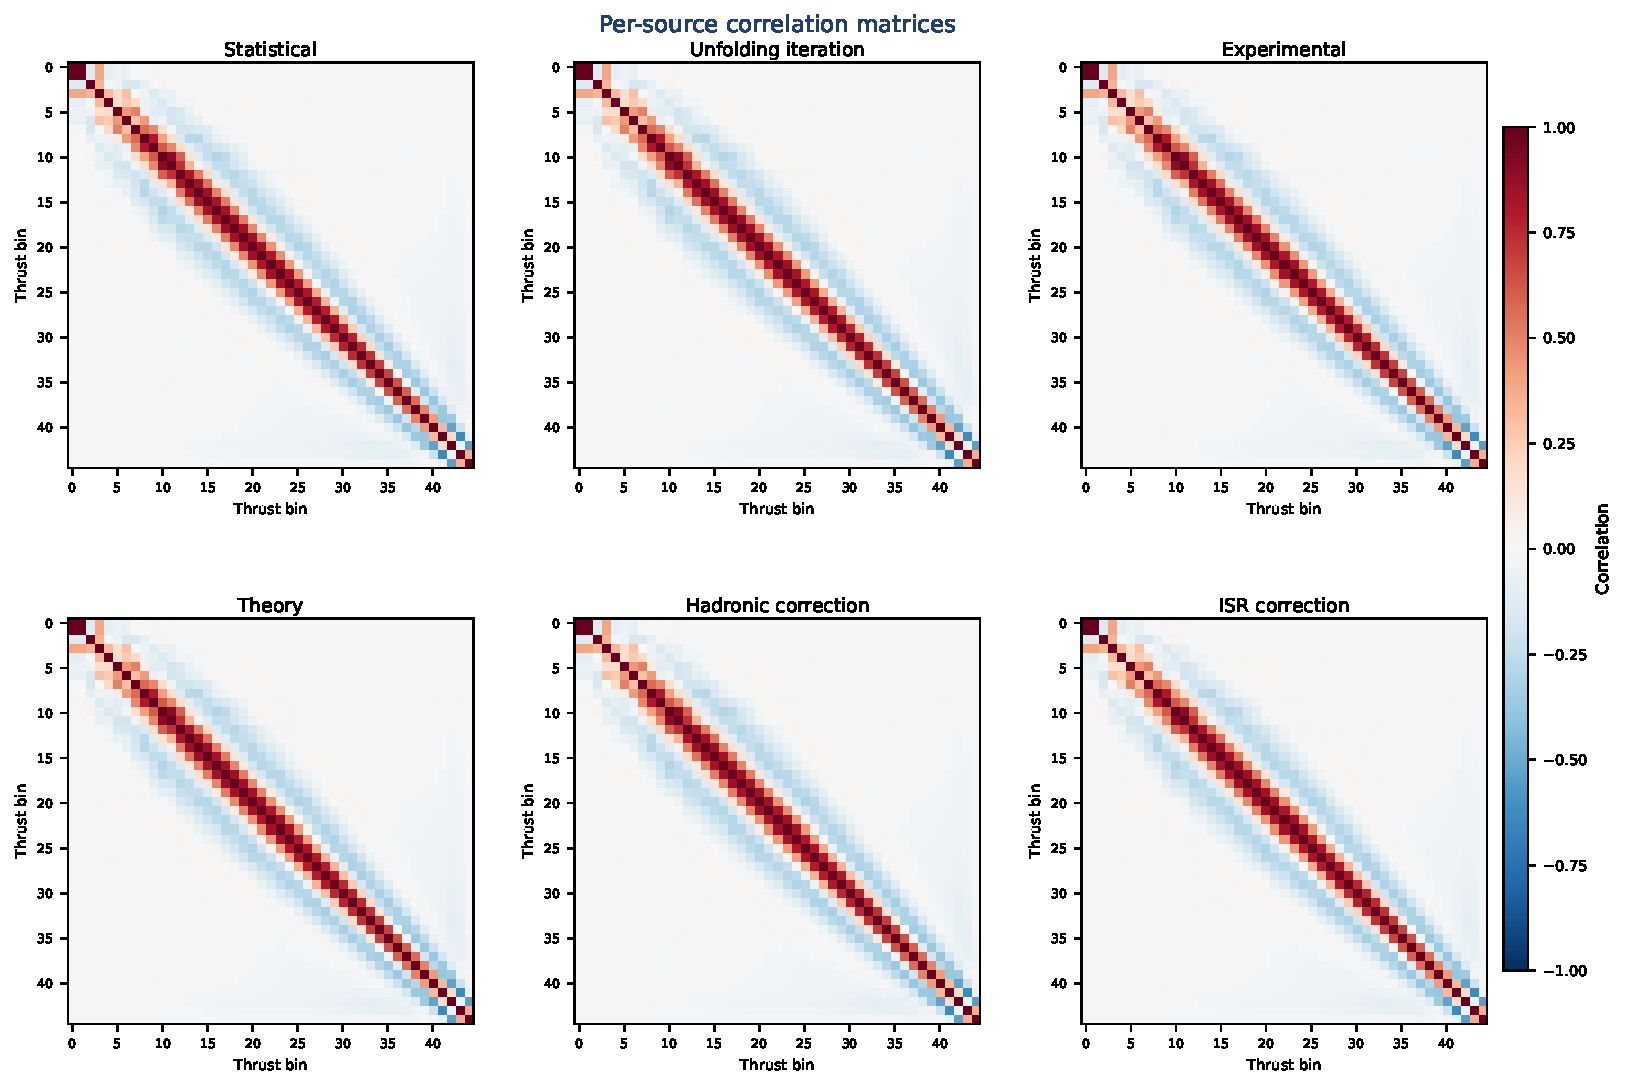
\includegraphics[width=\textwidth]{figures/corr_matrices_per_source.pdf}
\caption{Per-source correlation matrices for the six independent uncertainty
components: statistical (top left), unfolding-iteration (top center), experimental
(top right), theory (bottom left), hadronic correction (bottom center), and ISR
correction (bottom right). All matrices use the same color scale ($-1$ to $+1$,
red/blue). Under the nominal model the theory panel is diagonal (the identity), since
the theory uncertainty is a bin-wise generator envelope; the extended off-diagonal
structure resides in the statistical, iteration, and experimental panels and originates
from the unfolding of detector-level migration.}
\label{fig:corr_matrices_per_source}
\end{figure}

\FloatBarrier

\subsection{Per-source covariance matrices}
\label{sec:covariance_matrix}

The covariance matrices encode both the per-bin uncertainty magnitudes and the
bin-to-bin correlations for each source. The total covariance is the sum of all
six component covariances:
\begin{equation}
\mathrm{Cov}^{(\mathrm{tot})}_{ij} =
  \mathrm{Cov}^{(\mathrm{stat})}_{ij}
+ \mathrm{Cov}^{(\mathrm{iter})}_{ij}
+ \mathrm{Cov}^{(\mathrm{exp})}_{ij}
+ \mathrm{Cov}^{(\mathrm{theory})}_{ij}
+ \mathrm{Cov}^{(\mathrm{had})}_{ij}
+ \mathrm{Cov}^{(\mathrm{ISR})}_{ij}.
\end{equation}
Figure~\ref{fig:cov_matrices_per_source} shows the per-component covariance matrices;
Fig.~\ref{fig:cov_matrix_total} shows the total.

The component covariance magnitudes directly reflect the per-bin uncertainty sizes
shown in the breakdown plots of Sec.~\ref{sec:uncertainty_breakdown}. The theory
covariance (bottom left in Fig.~\ref{fig:cov_matrices_per_source}) has the largest
diagonal magnitude, reflecting the dominant theory envelope, but is diagonal by
construction under the nominal model and so has no off-diagonal structure. The most
extended off-diagonal structure is carried by the experimental covariance, whose
non-trivial off-diagonal entries are driven by the coherent neutral-response variations.
The statistical and iteration covariances are comparatively small; the ISR correction
produces a near-diagonal covariance consistent with its bin-local MC-statistical origin.

\begin{figure}[t!]
\centering
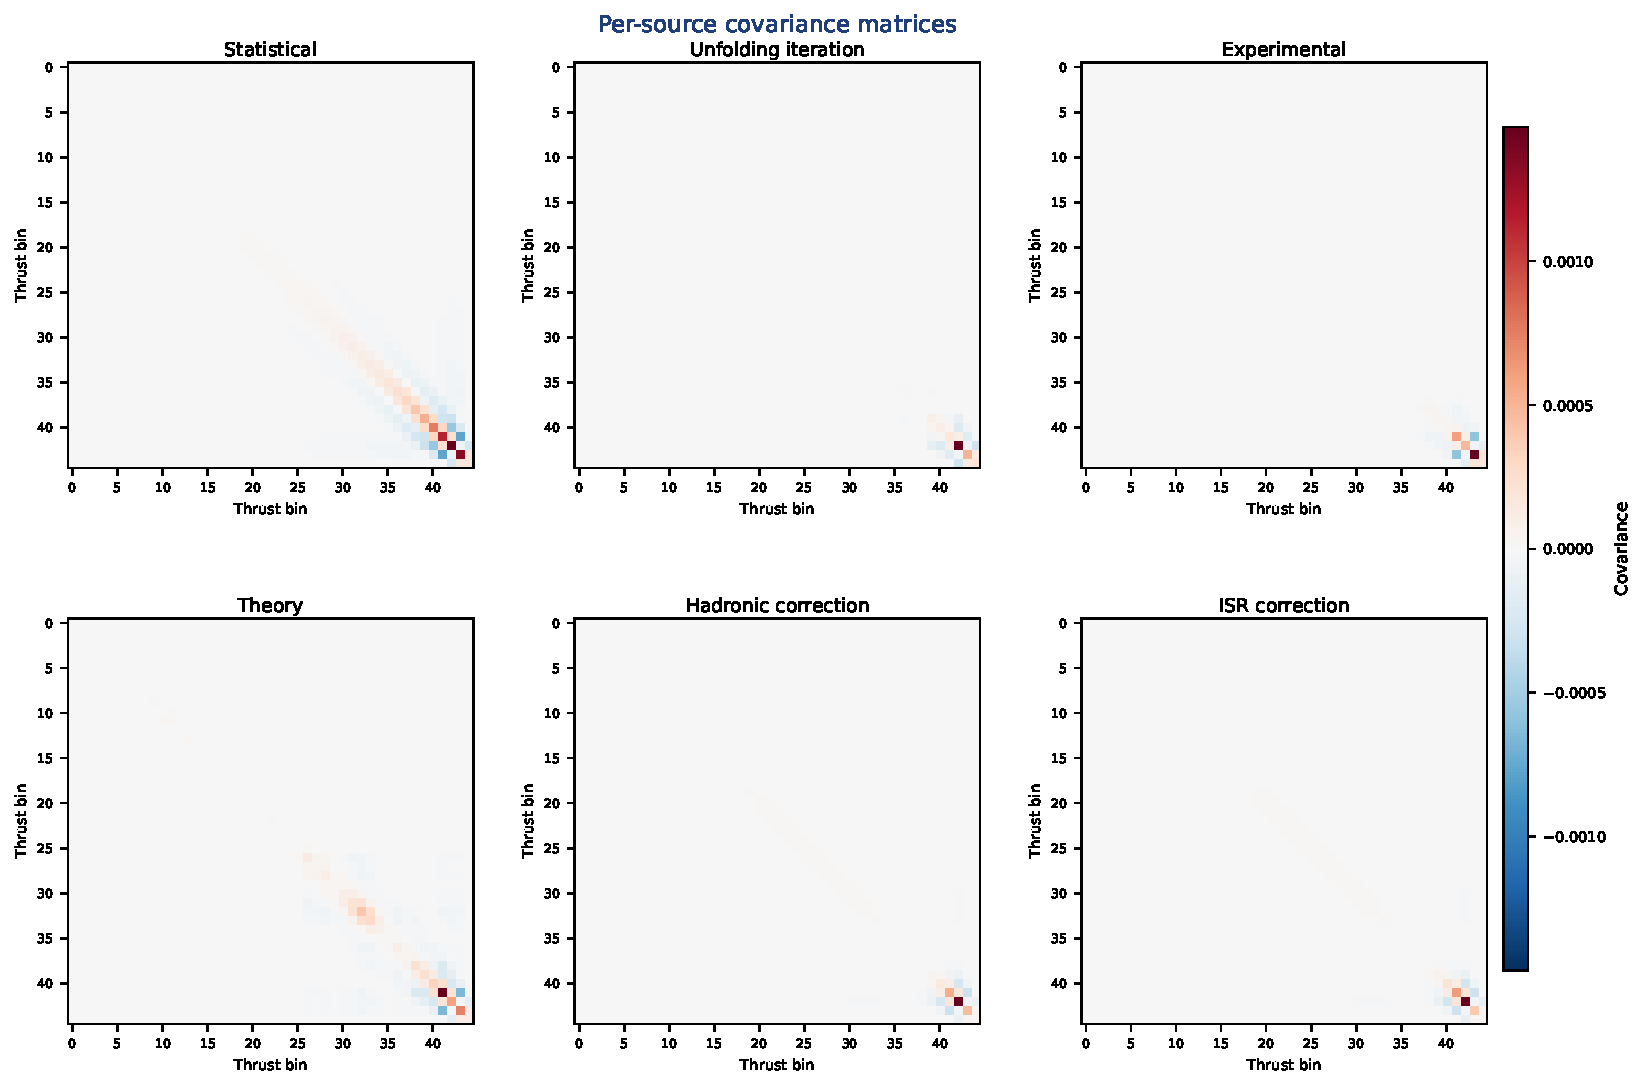
\includegraphics[width=\textwidth]{figures/cov_matrices_per_source.pdf}
\caption{Per-source covariance matrices for the six independent uncertainty
components: statistical (top left), unfolding-iteration (top center), experimental
(top right), theory (bottom left), hadronic correction (bottom center), and ISR
correction (bottom right). Each panel uses a symmetric color scale centered on zero
(red: positive, blue: negative). The theory component dominates the total covariance
in diagonal magnitude but is diagonal by construction under the nominal model; the
off-diagonal structure is carried by the experimental and statistical/unfolding
components.}
\label{fig:cov_matrices_per_source}
\end{figure}

The total covariance matrix (Fig.~\ref{fig:cov_matrix_total}) is the primary product
exported for theory use. Theory contributes the largest diagonal magnitude across the
central thrust range but, being diagonal under the nominal model, adds no off-diagonal
structure; the off-diagonal correlations come from the unfolding/response migration
(statistical covariance and the components that inherit its template) and from the
experimental component. Theory consumers are encouraged to use the fit-window total
covariance (covering $0.505\le T<1.00$, 45 bins) for $\alpha_s$ extractions rather
than the full-range matrix, to avoid the regions of large uncertainty and poor
MC-model control near the kinematic boundaries.

\begin{figure}[t!]
\centering
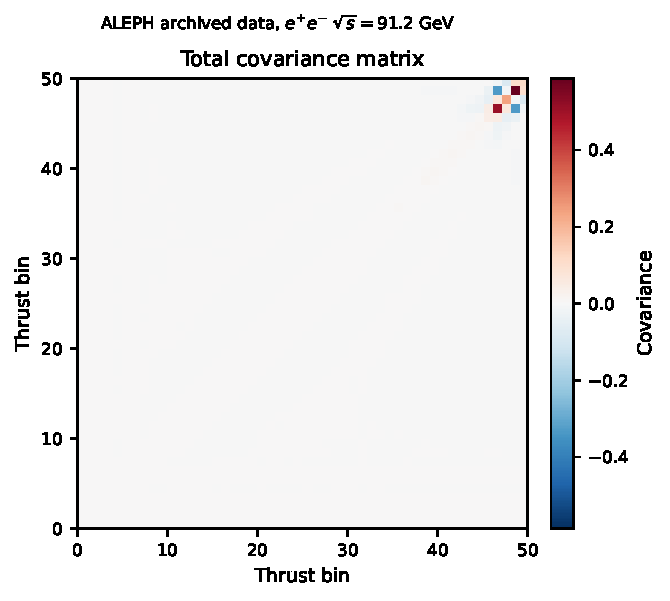
\includegraphics[width=0.72\textwidth]{figures/cov_matrix_total.pdf}
\caption{Total covariance matrix, combining all six uncertainty components.
Theory dominates the diagonal across the central thrust range but is diagonal under
the nominal model and adds no off-diagonal correlation; the off-diagonal structure
comes from the unfolding/response migration and the experimental component. The full
covariance matrix must be used in any downstream fit; diagonal uncertainties alone
would underestimate the true statistical power of the result. The fit-window version
($0.505\le T<1.00$) is recommended for $\alpha_s$ extractions.}
\label{fig:cov_matrix_total}
\end{figure}

\FloatBarrier
